% !TEXroot=main.tex
\section{Navigation}
{	
		Nachdem der Roboter nun auf der durch den Kartenserver bereitgestellten Karte verordnet wurde, muss dem Roboter ein Navigationsziel gegeben werden, damit eine Route zu diesem Punkt berechnet werden kann. Daraufhin soll der Roboter autonom zu diesem Punkt navigieren. Dieser Abschnitt stellt den letzten Schritt des Projekts dar.
		
		\subsection{Navigationsziel festlegen}
		{
			Rviz bietet dazu eine einfache Möglichkeit. In der oberen Leiste kann die Option ``\emph{2D Nav Goal}`` genutzt werden, um graphisch auf der vorliegenden Karte eine Zielposition festzulegen. Diese wird durch einen Pfeil repräsentiert und beinhaltet auch die Blickrichtung (Abbildung \ref{pic:rviznavgoalsmall}).
			\begin{figure}[b]
				\centering
				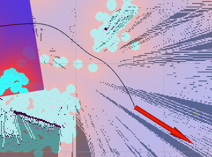
\includegraphics[height=5cm]{Bilder/rviz_navgoal_small.png}
				\caption{Eine in Rviz gesetzte Zielposition} 
				\label{pic:rviznavgoalsmall}
			\end{figure}
		Diese Position wird durch Rviz unter dem \emph{move\textunderscore base\textunderscore simple/goal}-Topic als Nachricht des  \emph{geometry\textunderscore msgs/PoseStamped}-Typs veröffentlicht und damit an die \emph{move\textunderscore base} weitergegeben.
		}
	
		\subsection{Implemention}
		{
			Die Navigation und Wegplanung geschieht durch das \emph{move\tus base}- Paket. Dabei wird zuerst, wie erwähnt, der grobe Weg, gefolgt von dem exakten Weg im lokalen Bereich berechnet.
		}
}	